\documentclass[oneside,final,14pt,a4paper]{extreport}

\usepackage{tempora} % Times New Roman alike font

\usepackage{vmargin}
\setpapersize{A4}
\setmarginsrb{2.5cm}{2.2cm}{2.2cm}{2.2cm}{0pt}{10mm}{0pt}{13mm}
\usepackage{setspace}
\setstretch{1.5}
\usepackage{indentfirst}
\parindent=1.25cm

%%%%% ADDED TO SUPPORT TT BOLD FACES %%%%
\DeclareFontShape{OT1}{cmtt}{bx}{n}{<5><6><7><8><9><10><10.95><12><14.4><17.28><20.74><24.88>cmttb10}{}
\renewcommand{\ttdefault}{pcr}
%%%%% END %%%%%%%%%%%%%%%%%%%%%%%%%%%%%%%

\usepackage{atbegshi,picture}
\usepackage[T1,T2A]{fontenc}
\usepackage[utf8]{inputenc}

\usepackage[english]{babel}
\usepackage[backend=biber,style=ieee,autocite=inline]{biblatex}
\bibliography{thesis.bib}
\DefineBibliographyStrings{english}{%
bibliography = {References},}
\usepackage{blindtext}

\usepackage{pdfpages}
\newenvironment{bottompar}{\par\vspace*{\fill}}{\clearpage}
\usepackage{amsmath,amsfonts}
\usepackage{url}
\usepackage{amsthm}
\newtheorem{theorem}{Theorem}
\newtheorem{corollary}{Corollary}
\newtheorem{lemma}{Lemma}
\newtheorem{proposition}{Proposition}
\theoremstyle{definition}
\newtheorem{definition}{Definition}
\theoremstyle{remark}
\newtheorem*{remark}{Remark}
\theoremstyle{remark}
\newtheorem*{example}{Example}

\usepackage{float}
\usepackage{graphicx}
\graphicspath{{figs/}} %path to images
\usepackage{array}
\usepackage{multirow,array}
\usepackage{caption}
\usepackage{subcaption}
\usepackage{hyperref}
\hypersetup{colorlinks=true, linkcolor=black, citecolor=black}
\usepackage{paralist}
\usepackage{listings}
\usepackage{zed-csp}
\usepackage{fancyhdr}
\usepackage{csquotes}
\usepackage{color}
\usepackage{anyfontsize}
\usepackage{mathptmx}
\usepackage{t1enc}
\usepackage{dirtytalk}

\usepackage{chngcntr}
\usepackage{upgreek}
\usepackage{bm}
\usepackage{hyperref}
\usepackage{booktabs}
\usepackage{multirow}
\usepackage{longtable}
\usepackage[font=singlespacing, labelfont=bf]{caption}
%Hints
\newcommand\pic[1]{(Fig. \ref{#1})} %Ref on figure
\newcommand\tab[1]{(Tab. \ref{#1})} %Ref on table

\setlength{\headheight}{32.0976pt}
\usepackage{enumitem}
\newlist{inlinelist}{enumerate*}{1}
\setlist*[inlinelist,1]{%
label=(\arabic*),
}

% \setcounter{secnumdepth}{4}
\captionsetup[table]{labelfont={normalfont}, name={TABLE}, labelsep={newline}}
\setlength{\parindent}{2em}
\DeclareCaptionLabelSeparator{figSep}{.\quad}
\captionsetup[figure]{labelfont={normalfont}, name={Fig.}, labelsep=period}
\counterwithin{figure}{chapter}

\usepackage{titlesec}
\titleformat{\section}[hang]{\fontsize{20}{24}\selectfont\filcenter}{\Roman{section}}{1em}{}
\titleformat{\subsection}[hang]{\itshape}{\Alph{subsection}.}{1em}{}[]
\titleformat{\subsubsection}[runin]{\itshape}{\arabic{subsubsection})}{1em}{}[$:$]
\titlespacing{\subsubsection}{1em}{1em}{1em}
\titleformat{\paragraph}[runin]{\itshape}{\alph{paragraph})}{1em}{}[$:$\quad]
\titlespacing{\paragraph}{2em}{1em}{1em}

\usepackage{placeins} % for \FloatBarrier

\pagestyle{fancyplain}

% remember section title
\renewcommand{\chaptermark}[1]%
{\markboth{\chaptername~\thechapter~--~#1}{}}

% subsection number and title
\renewcommand{\sectionmark}[1]%
{\markright{\thesection\ #1}}

\rhead[\fancyplain{}{\bf\leftmark}]%
{\fancyplain{}{\bf\thepage}}
\lhead[\fancyplain{}{\bf\thepage}]%
{\fancyplain{}{\bf\rightmark}}
\cfoot{} %bfseries

\usepackage{pgfplots}
\pgfplotsset{width=14cm, height=14cm, compat=1.18}

\DeclareFixedFont{\ttb}{T1}{txtt}{bx}{n}{12} % for bold
\definecolor{deepblue}{rgb}{0,0,0.5}
\definecolor{deepurple}{rgb}{0.5,0,0.3}
\definecolor{deepgreen}{rgb}{0,0.5,0}
\definecolor{halfgray}{RGB}{250, 250, 250}

\lstset{
	language=Python,
	columns=fullflexible,
	tabsize=4,
	keywordstyle=\ttb\color{deepblue},
	emph={self},
	emphstyle=\color{deepurple},
	keywordstyle=\ttb\color{deepblue},
	stringstyle=\color{deepgreen},
	showstringspaces=false,
 	backgroundcolor=\color{halfgray},
 	frame=tb,
 	xleftmargin=5mm,
 	aboveskip=5mm,
 	framexleftmargin=5mm,
}


\newcommand{\dedication}[1]
{\thispagestyle{empty}

\begin{flushleft}\raggedleft #1\end{flushleft}
}

\begin{document}

% 
\includepdf[pages=-]{title.pdf}

\includepdf[pages=-, offset=75 -75]{title.pdf}
% 
\includepdf[offset=1in -1in,noautoscale, pages=-]{title.pdf}

\tableofcontents
\listoftables
\listoffigures
\newpage


\begin{abstract}

The rapid development of software and its increasing integration into various aspects of our daily lives have brought about unprecedented challenges in ensuring its security. With the convergence of the non-IT and IT industries, the number of software errors and vulnerabilities has increased, posing significant risks to individuals, organizations, and society as a whole. Despite continuous efforts to improve cybersecurity, the omnipresence of cyber threats and the lack of a single foolproof method to ensure software correctness persist as pressing concerns.

This thesis project aimed to address the critical need for enhanced cybersecurity by investigating the potential of Metamorphic Testing and Combinatorial Testing as effective techniques to identify and mitigate software vulnerabilities. The research sought to evaluate the combined use of these methods and evaluate their efficiency, effectiveness, and comprehensive coverage in detecting security flaws.

To achieve the research objective, a rigorous study design was employed, focusing on the application of Metamorphic Testing and Combinatorial Testing to diverse software systems and scenarios. The study design incorporated various black-box testing techniques, including Domain Testing, Boundary Value Analysis, and the utilization of Metamorphic Relations to address the Test Oracle Problem. Extensive experimentation and analysis were performed to assess the benefits and limitations of this combined approach.

The research project yielded substantial findings, demonstrating that the integration of Metamorphic and Combinatorial Testing techniques significantly improved the efficiency and quality of software security testing. The approach exhibited superior coverage of potential vulnerabilities and offered a more comprehensive understanding of software behavior under various conditions.

The contribution of this work lies in providing a robust framework for improving cybersecurity through the synergistic use of Metamorphic and Combinatorial Testing. The results have direct applicability in industry and academia, offering a practical strategy to identify and address software vulnerabilities more effectively. This research contributes to advancing the state-of-the-art in cybersecurity and provides valuable insights into safeguarding the integrity and reliability of software systems in an increasingly interconnected world.

\end{abstract}
\setcounter{page}{8}
% set manually the number, from which Chapter 1 starts!
% Why do we put 7 in this case?
% Title page - page 1
% Contents - page 2, page 3
% List of tables - page 4
% List of figures - page 5
% Abstract - page 6
% Chapter 1 - page 7
% In your thesis the counter number can be different, please count carefully and insert the corresponding number.

\chapter{Introduction}
\label{chap:intro}

\section{Motivation}

% Rapid development of software led to Increasing number of software errors and vulnerabilities. Number of CVE per year increasing \cite{CVE}. Need for Enhanced Cybersecurity using automated testing methods. Using CI practices became standard in industry. Automated tests need to be fast so they can find bugs and vulnerabilities at the early stages of development. Existing techniques such as code analysis, fuzzing, domain testing. Need for more efficient and effective techniques. Proposed method of combining metamorphic testing and combinatorial testing. Semi automated approach to generate test cases. Small number of tests due to nature of combinatorial testing. More efficient because of metamorphic testing.

In recent years, the rapid evolution of software development has resulted in a significant surge in software errors and vulnerabilities. The escalating number of Common Vulnerabilities and Exposures (CVEs) reported each year reflects the growing challenges faced in ensuring the security and reliability of software systems \cite{CVE}. As the digital landscape becomes increasingly complex and interconnected, the need for robust cybersecurity measures has become paramount.

The traditional approaches to software testing are often inadequate in detecting and mitigating vulnerabilities effectively. With the adoption of Continuous Integration practices as a standard in the industry, there's a heightened demand for automated testing methods that can seamlessly integrate into the development workflow. The primary objective is to identify and address bugs and vulnerabilities at the earliest stages of the software development life cycle.

Several techniques have been employed to enhance software testing and security, including but not limited to code analysis, fuzzing, and domain testing. While these methods have proven to be valuable, there remains a pressing need for more efficient and effective approaches to bolster cybersecurity measures.

\section{Proposed Approach}

This thesis proposes a novel methodology that combines two distinct testing techniques: metamorphic testing and combinatorial testing. The proposed approach adopts a semi-automated methodology for generating test cases. By leveraging both metamorphic and combinatorial testing principles, the aim is to streamline the testing process while ensuring adequate coverage of the system under test. This hybrid approach strikes a balance between manual intervention and automated testing, optimizing the efficiency and effectiveness of the testing process.

One of the key advantages of the proposed method is its ability to achieve comprehensive test coverage with a relatively small number of test cases. Combinatorial testing, by systematically exploring the interaction of input parameters, helps in reducing the number of test cases required. Meanwhile, metamorphic testing enhances the efficiency of the testing process by leveraging the inherent properties of the system.

\section{Terminology}

This section presents an overview of key concepts in the field of metamorphic and combinatorial testing, focusing on their applications in cybersecurity. The definitions below lay the groundwork for understanding the methodologies discussed in subsequent sections.

\subsection{Black Box Testing}

\textbf{Black Box Testing} is a methodology where the internal workings or implementation details of the system under test are not known or considered by the tester. Testing is based solely on defined specifications or thought specs. Black-box testing relies only on the input/output behavior of the software \cite{Testing}.

Some examples of black-box testing techniques include:
\begin{itemize}
    \item Metamorphic Testing
    \item Combinatorial Testing
    \item Fuzz Testing
    \item Boundary Value Analysis
\end{itemize}

\subsection{Metamorphic Testing}

\textbf{Metamorphic Testing} is an effective technique for alleviating the oracle problem, testing "untestable" programs where failures are not revealed by checking individual outputs, but by checking expected relations among multiple executions of the program under test \cite{CybersecurityMT}.

\textbf{Metamorphic Relation (MR)} is a property or characteristic that should be maintained between multiple test case outputs. If an MR is violated, it suggests a potential defect in the software \cite{MetamorphicTestingReview}.

\textbf{Metamorphic Group (MG)} is a multiple sequence of inputs related to each other by a particular metamorphic relation. It consists of a sequence of source inputs and follow-up inputs \cite{MetamorphicTestingReview}. \textit{Example:} \textit{MR1: $f(x, y) = f(y, x)$} is a metamorphic relation, and \textit{MG1: {1, 2} $\rightarrow$ {2, 1}} is a metamorphic group.

\subsection{Combinatorial Testing}

\textbf{Combinatorial Testing} is a software testing technique that focuses on testing subsets of combinations of input values and preconditions to uncover defects. It's particularly effective when the number of parameters and their possible values is too large for exhaustive testing \cite{FELDERER20161}.

Consider a function $f(a, b, c)$ with boolean parameters.

\textbf{Test Case} is a set of conditions or variables under which a tester will determine whether a system under test satisfies requirements or works correctly \cite{comer}. For our function $f(a, b, c)$, a test case could be \textit{a = 1, b = 0, c = 1}.

\textbf{t-way combination} is a set of t input values, one from each of t input parameters \cite{comer}. For our function $f(a, b, c)$, a 2-way combination could be \textit{a = 1, b = 0}.

\textbf{t-way covering array} is a set of t-way combinations that covers all t-way combinations of input values. It is used to ensure that all combinations of input values are tested at least once. Fig. \ref{fig:CovArray} shows a covering array for $f(a, b, c)$ with 2-way combinations.

\begin{figure}
\centering
\begin{tabular}{|c|c|c|}
    \hline
    a & b & c \\
    \hline
    0 & 0 & 0 \\
    0 & 1 & 1 \\
    1 & 0 & 1 \\
    1 & 1 & 0 \\
    \hline
\end{tabular}
\caption{Covering array for $f(a, b, c)$ with 2-way combinations. Notice, that each 2 columns contain all possible combinations of 0's and 1's.}
\label{fig:CovArray}
\end{figure}

\subsection{Other Testing Techniques}

\textbf{Fuzz Testing} is a technique involving providing invalid, unexpected, or random data as input to a computer program. The program is then monitored for exceptions such as crashes or failing built-in code assertions, or for finding potential memory leaks \cite{Fuzz}.

\textbf{Boundary Value Analysis (BVA)} is a software testing technique in which tests are designed to include representatives of boundary values. It is based on the idea that input values at the extreme ends of the input domain are more likely to cause errors in the system \cite{BVA}.

\textbf{Property-based Testing} is a software testing technique that involves checking whether a system satisfies a set of properties, which are logical assertions about the system's behavior. It is a form of black-box testing, where the tester specifies the properties that the system should satisfy, but does not specify how the system should satisfy them \cite{Hypothesis}. \textit{Metamorphic Testing} is a form of property-based testing.

\subsection{General Testing Terms}

\textbf{Oracle Problem} is a problem in software testing where the tester does not know the correct output for a given input, and thus cannot determine if the system under test has passed or failed the test \cite{FELDERER20161}.

\textbf{System Model} is a model of the system under test (SUT) and/or its environment built from informal requirements, existing specification documents, or the SUT itself. It is used as input for automated test generation \cite{FELDERER20161}.

\textbf{Test Suite} is a collection of test cases that are used to test a software program to show that it has some specified set of behaviors.

\subsection{Cybersecurity}

\textbf{Cybersecurity} is the protection of computer systems and networks from information disclosure, theft of or damage to their hardware, software, or electronic data, as well as from the disruption or misdirection of the services they provide \cite{FELDERER20161}.

\textbf{Cybersecurity Testing} is for testing software system requirements related to security properties like confidentiality, integrity, availability, authentication, authorization, and non-repudiation. It involves techniques such as penetration testing, fuzz testing, static and dynamic analysis to identify vulnerabilities \cite{FELDERER20161}.

\subsection{Test Metrics}

\textbf{Test Metrics} are used to measure the effectiveness of the testing process. They are used to monitor the progress of testing, assess the quality of the software, and identify areas for improvement.

\textbf{Test Coverage} is a measure used to describe the degree to which the source code of a program is executed when a particular test suite runs. Some categorizations of test coverage provided below:

\begin{itemize}
    \item \textbf{Statement Coverage} measures the number of statements in the source code that have been executed by a test suite.
    \item \textbf{Branch Coverage} measures the number of if conditions, jumps, etc., in the source code that have been executed by a test suite.
    \item \textbf{Weak Coverage} means that the test suite has executed at least one of the possible paths through the code.
    \item \textbf{Strong Coverage} means that the test suite has executed all possible paths through the code.
\end{itemize}


\section{Structure of the Thesis}

This thesis is organized as follows:

\begin{itemize}
    \item \textbf{Introduction}: Provides an overview of the research problem, objectives, and proposed methodology.
    \item \textbf{Literature Review}: Surveys the existing literature on software testing techniques, cybersecurity, and the principles of metamorphic and combinatorial testing.
    \item \textbf{Methodology}: Details the proposed approach, including the integration of metamorphic and combinatorial testing, and the semi-automated test case generation process.
    \item \textbf{Implementation}: Describes the implementation of the proposed methodology and presents the results of empirical experiments conducted to evaluate its efficacy.
    \item \textbf{Evaluation and Discussion}: Analyzes the findings of the experiments and discusses their implications for software testing and cybersecurity.
    \item \textbf{Conclusion}: Summarizes the key findings of the research and outlines potential avenues for future research in this area.
\end{itemize}


% \begin{figure}[hbt]
% \centering
% 
\includegraphics[]{figs/inno.png}
% \caption{One kernel at $x_s$ (\emph{dotted kernel}) or two kernels at
% $x_i$ and $x_j$ (\textit{left and right}) lead to the same summed estimate
% at $x_s$. This shows a figure consisting of different types of
% lines. Elements of the figure described in the caption should be set in
% italics, in parentheses, as shown in this sample caption.}
% \label{fig:example}
% \end{figure}

% This is a table:
% % currsize is not set in the long table environment, so we need to set it before we set it up.
% \makeatletter
% \let\@currsize\normalsize
% \makeatother
%
% % tabular environments are set to be single-spaced in the  thesis class,  but long tables do not use tabular
% % to get around this, set the spacing to single spacing at the start of the long table environment, and set it back to double-spacing at the end of it
%
% \begin{longtable}{c|c|c}
% \caption[This is the title I want to appear in the List of Tables]{This Is a Table Example} \label{tab:pfams} \\
% \hline
% A & B & C \\
% \hline
% \endfirsthead
% \multicolumn{3}{@{}l}{} \\
% \hline
% A & B & C\\
% \hline
% \endhead
% a1 & b1 & c1 \\
% a2 & b2 & c2\\
% a3 & b3 & c3\\
% a4 & b4 & c4\\
% \hline
% \end{longtable}

% The package ``upgreek'' allows us to use non-italicized lower-case greek letters. See for yourself: $\upbeta$, $\bm\upbeta$, $\beta$, $\bm\beta$. Next is a numbered equation:
% \begin{align}
% \label{eq:name}
% \|\bm{X}\|_{2,1}={\underbrace{\sum_{j=1}^nf_j(\bm{X})}_{\text{convex}}}=\sum_{j=1}^n\|\bm{X}_{.,j}\|_2
% \end{align}
% The reference to equation (\ref{eq:name}) is clickable.
% \section[Theorems, Corollaries, Lemmas, Proofs, Remarks, Definitions and Examples]{Theorems, Corollaries, Lemmas, Proofs, Remarks, Definitions,and Examples}






%!TEX root = ../thesis.tex

\chapter{Literature Review}
\label{ch:lr}

Cybersecurity threats require innovative testing methods to ensure the reliability and security of the software. This literature review delves into the current state-of-the-art in Combinatorial Testing (CT) and Metamorphic Testing (MT) for cybersecurity, explores the integration of CT and MT, and assesses the efficiency of these methods working together and their potential applications in cybersecurity.


\section{Criteria and Process}\label{sec:criteria-and-process}

The selection and analysis of literature for this review were guided by specific criteria and a structured process. Search keywords included "Combinatorial Testing in Cybersecurity," "Metamorphic Testing in Cybersecurity," and "Integration of CT and MT in Cybersecurity." The search was conducted across multiple academic databases, including IEEE Xplore, ACM Digital Library, and Google Scholar. Articles were chosen based on the number of citations, the date of publication, the popularity of the journal, and relevance to the topic. The method involved a critical review of selected articles, focusing on their methodologies, findings, and implications in the context of cybersecurity testing.


\section{Combinatorial Testing in Cybersecurity}\label{sec:combinatorial-testing-in-cybersecurity}

Within the cybersecurity domain, Combinatorial Testing has been effectively utilized, particularly in generating test cases aimed at identifying vulnerabilities like SQL injection \cite{Simos2019SQL} and XSS injections \cite{Garn2014XSS}. The focus of both studies was primarily on a singular type of vulnerability. These investigations have demonstrated that Combinatorial Testing is both rapid and efficient in uncovering vulnerabilities. However, it is important to note that the scope of these studies is somewhat restricted in terms of the range of technologies evaluated.


\section{Metamorphic Testing in Cybersecurity}\label{sec:metamorphic-testing-in-cybersecurity}

The literature on Metamorphic Testing (MT) in cybersecurity provides insightful perspectives on its application and effectiveness. Segura \textit{et al.} highlight the fundamental concept of MT to overcome the oracle problem in software testing, where the correctness of the output is ambiguous \cite{CybersecurityMT}. This aspect is particularly crucial in cybersecurity, where accurate results are essential but often difficult to define.

In their exploration of MT's application to cybersecurity, researchers have demonstrated its efficacy in detecting hidden bugs in vital applications. A notable example is the testing of compilers and code obfuscators, where traditional testing methods may fail \cite{CybersecurityMT} \cite{GLSLFuzz}. The use of MT in such scenarios underlines its ability to handle complex and critical software systems.

The development and implementation of the METRIC framework \cite{ChenPoon2016} mark a significant advancement in MT. This approach systematically identifies metamorphic relations (MRs) through a category-choice framework, simplifying the process of MR identification which was previously manual and ad hoc. This systematic approach is particularly advantageous in cybersecurity, where the generation of reliable test oracles is challenging. Iakusheva et al. showed that MR derivation can be further simplified by using domain specific guidelines \cite{MetaRU}.

MT's role in cybersecurity extends to various practical applications.
It facilitates negative testing and the evaluation of security-related functionalities, often problematic with conventional testing methods. A case in point is the use of MT in identifying vulnerabilities such as the Heartbleed bug in OpenSSL, demonstrating its ability to handle complex real-world cybersecurity issues \cite{OpenSSLMT}.


\section{Integration of Combinatorial and Metamorphic Testing}\label{sec:integration-of-combinatorial-and-metamorphic-testing}

The combination of Combinatorial Testing (CT) and Metamorphic Testing (MT) is explored by Niu \textit{et al.} \cite{comer} in an innovative approach to software testing. Their study tackles the challenge in CT related to the creation of automated test oracles, a problem that often leads to manual and error-prone processes in testing.

Niu \textit{et al.} introduce a new method called COMER, which blends MT with CT. This method focuses on forming pairs of test cases, known as Metamorphic Groups (MGs), based on specific metamorphic relations (MRs). These MGs allow for automatic checking of test results by verifying if the outputs go against the MRs.


\section{Conclusion}\label{sec:conclusion}

The exploration of Combinatorial Testing (CT) and Metamorphic Testing (MT) within cybersecurity, as outlined in this literature review, lays the groundwork for advancing the field of software testing. Although these methodologies have been examined separately in various contexts, their integration, especially in addressing cybersecurity challenges, opens new avenues for research. The innovative approach of combining CT and MT, as proposed by Niu \textit{et al.} \cite{comer}, demonstrates a promising direction towards automating and enhancing the accuracy of testing processes. This research seeks to build on these foundational studies, focusing on the implications and practical applications of integrating CT and MT in the domain of cybersecurity, a critical area that has not been fully explored in the existing literature.

\newpage

\chapter{Methodology}
\label{chap:met}

This study employs the COMER methodology for the generation of test cases. In order to assess the efficacy of the framework and conduct comparative analyses with other existing frameworks, I undertook the task of implementing it from scratch using the Python programming language. The initial implementation by Niu \textit{et al.} \cite{comer} was coded in Java. However, this implementation presented certain limitations; the code was compiled into a jar file, making it challenging to extend or modify functionalities. Consequently, I opted to develop my own implementation in Python, making necessary modifications to facilitate experimentation with different datasets and enhancing the usability of the framework. Python was chosen due to its user-friendly syntax and the availability of extensive libraries for data manipulation and visualization.

\section{COMER Framework}

The COMER framework serves the purpose of generating test cases, leveraging both traditional Combinatorial Testing (CT) methods and incorporating metamorphic relations during the generation process. Upon receiving inputs including a set of metamorphic relations, a set of constraints, and abstract input parameters, COMER generates test cases that adhere to the specified constraints while satisfying certain metamorphic relations.

The framework operates in two primary stages:

\subsection{Abstract Test Case Generation}

The algorithm for abstract test case generation encompasses two main pathways. At each step, there exists a probability distribution determining the choice between two flows. In the first flow, the algorithm functions akin to a conventional CT generation algorithm, employing a greedy approach to generate test cases until achieving the desired t-way coverage. Conversely, the second flow involves the selection of a previously generated test case, followed by the generation of subsequent test cases utilizing metamorphic relations.

\subsection{Concrete Test Case Generation}

Subsequently, the generated abstract test cases are mapped to concrete ones. For test cases generated via CT methods, the concrete test case is produced by randomly selecting a value from the domain corresponding to the abstract value. Conversely, for test cases generated through metamorphic relations, the framework utilizes the specified metamorphic relation to generate subsequent test cases.

\begin{figure}[hbt]
\centering
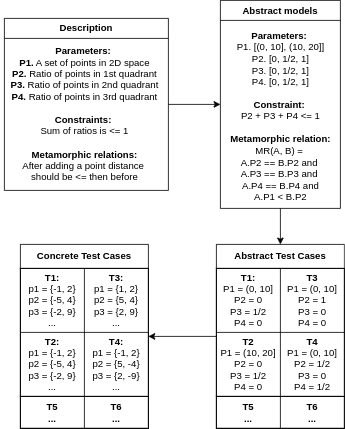
\includegraphics[]{figs/test_cases.png}
\caption{Example of generating test cases for \textit{FindClosest} function. Note that $T1$ and $T2$ are parameters generated by utilizing MR.}
\label{fig:secex}
\end{figure}

\section{Limitations}

Despite the advancements made in the original COMER implementation, certain limitations were identified. Firstly, the reliance on a greedy approach for generating Combinatorial Testing (CT) test cases posed a notable drawback. While this method can increase the speed of generation process, it may result in an excessive number of test cases, potentially compromising efficiency and resource utilization. Secondly, the focus of the implementation solely on metamorphic relations with a single input and a single follow-up test case restricted its applicability to scenarios involving more complex MRs. Thirdly, the lack of provision for generating test cases for functions beyond those already supported in the implementation posed a significant constraint.

In my implementation, efforts were made to mitigate some of these limitations. To overcome the limitation of supporting only a limited range of functions, I worked to improve the framework by allowing the generation of test cases for any function. Additionally, in response to concerns regarding the effectiveness of the greedy approach, provisions were made to incorporate alternative algorithms for CT test case generation, thereby offering users flexibility in selecting the most suitable approach. However, it is important to note that the limitation pertaining to MRs with multiple inputs and follow-up test cases remains unaddressed in my implementation, representing an area for potential future research and improvement.

%!TEX root = ../thesis.tex

\chapter{Implementation}
\label{ch:impl}

This section outlines how I created my version of the COMER framework.
Additionally, it presents the outcomes of test executions and compare it to the original Java COMER framework implementation.

\section{Details of Implementation}\label{sec:details-of-implementation}

The implementation is encapsulated within a Python library, which can be seamlessly installed via the Python package manager, pip.
This library facilitates testing procedures by requiring input parameters, constraints, metamorphic relations and producing concrete test cases.
Library can be integrated with popular Python testing frameworks like Pytest and Unittest.
Under the hood, the library utilizes the \textit{python-constraint} package, which is a Python constraint solver.
The main function responsible for generating test cases is as follows:

\begin{lstlisting}[language=Python,label={lst:lstlisting}]
def generate_candidates(
    mr: Callable, p: list[list[int]],
    c: list[Callable], pca: list[list[int]],
    rep: int,  pr: float) -> list[list[int]
]:
    """Generates a set of candidate test cases."""
    candidates = []
    r = random.random()
    if r <= pr:
        tpre = rand_select(pca)
        for _ in range(rep):
            t = csp_solver(mr, tpre, p, c)
            candidates.append(t)
    else:
        for _ in range(rep):
            t = random_testcase(p, c)
            candidates.append(t)
    return candidates

\end{lstlisting}

The function adheres to the foundational principles of the COMER framework.
Specifically, based on a given probability, $pr$, function choose either Combinatorial Testing (CT) or Metamorphic Testing (MT) based approach.
In CT, it uses a Constraint Satisfaction Problem (CSP) solver to generate test cases iteratively.
In MT, it selects an existing test case from the provided pool ($pca$) and generates subsequent test cases using the CSP solver.

\section{Evaluation}\label{sec:evaluation}

To evaluate the efficacy of my implementation of the COMER framework, I conducted a series of experiments comparing its performance with the original Java implementation by Niu \textit{et al.} \cite{comer}.
The experiments focused on assessing the framework's ability to generate test cases accurately and efficiently across various scenarios.

%!TEX root = ../thesis.tex

\chapter{Evaluation and Discussion}
\label{ch:eval}

This chapter presents the outcomes of test executions and compare it to the original Java COMER framework implementation, as well as to CT approach. For this research, I formulated following research questions:

\begin{itemize}
  \item \textbf{RQ1:} How does the COMER framework compare to traditional Combinatorial Testing (CT) methods in terms of test case generation efficiency?
  \item \textbf{RQ2:} Can COMER be used to identify vulnerabilities in complex cybersecurity software more effectively than traditional CT methods?
  \item \textbf{RQ3:} Can this integrated technique be standardized into a framework or toolset for automated security testing?
  \item \textbf{RQ4:} Can relevant metamorphic relations and test pairs be systematically generated for complex cybersecurity software? Or does it require domain expertise?
\end{itemize}

\section{Evaluation}
\label{sec:evaluation}

To evaluate the efficacy of my implementation of the COMER framework, I conducted a series of experiments comparing its performance with the original Java implementation by Niu \textit{et al.} \cite{comer}.
The experiments focused on assessing the framework's ability to generate test cases accurately and efficiently across various scenarios.

Charts below present the results of the experiments conducted on the COMER framework. The experiments were conducted on the following injection types: SQL Injection on DVWA, SQL Injection on Web Goat, Blind SQL Injection on  Web Goat, and Form Sanitization in login forms. The injection were selected based on the large potential number of errors that could be uncovered and the complexity of the injection, including MR complexity and the number of test cases generated. Also, I choose to include Quicksort as a target for testing because original paper used it in its evaluation. All targets are described in Table~\ref{fig:injections}.

For the SQL injections I used Metamorphic Relations (MRs) to generate test cases. The MRs were designed to simulate various injection attack scenarios, such as UNION injections, where we try to add additional rows to the resulting SELECT, Condition injections, where we try to modify condition check to always be True, and string escape, there we specifically try to escape strings. All of the relations were used to either add a constant to input or reverse some part of the input.

The results are shown in the three charts, presenting number of test cases generated in Fig.~\ref{fig:test_cases}, number of faults detected in Fig.~\ref{fig:faults}, and execution time in seconds in Fig.~\ref{fig:exec_time}. The results are considered for three different scenarios: COMER with 75\% probability of selecting MR approach, COMER with 50\% probability of selecting MR approach, COMER with 25\% probability of selecting MR approach, and traditional CT approach using AllPairs algorithm. The selection of such scenarios allows to evaluate the difference between the traditional CT approach and the COMER framework, as well as the impact of the MR approach selection probability on the results.

\begin{table}[htbp]
  \centering
  \caption{Target Descriptions}
  \begin{tabular}{lrrr}
    \toprule
    Target & Domain size & MRs & Vulnerabilities \\
    \midrule
    Quicksort & $3^6$ & $3$ & $0$ \\
    SQL DVWA & $2^8*3*5*8$ & $3$ & $6$ \\
    SQL Web Goat & $2^7*6*10$ & $3$ & $6$ \\
    SQL Blind Web Goat & $2^7*6*10$ & $3$ & $6$ \\
    Form Sanitization & $2^{11} * 4^2$ & $2$ & $3$ \\
    \bottomrule
  \end{tabular}
  \label{fig:injections}
\end{table}

\begin{figure}[!t]
    \centering
    \begin{tikzpicture}
        \begin{axis}[
            ylabel={Number of Test Cases},
            ybar=0pt,
            bar width=10pt,  % Adjusts th;e gap between bar groups
            ymajorgrids=true,
            grid style=dashed,
%             legend pos=north west,
            symbolic x coords={SQL DVWA, SQL Web Goat, SQL Blind Web Goat, Form Sanitization, Quicksort},
            xtick=data,
            x tick label style={rotate=45, anchor=east},
        ]

        \addplot coordinates {
            (SQL DVWA, 142)
            (SQL Web Goat, 155)
            (SQL Blind Web Goat, 156)
            (Form Sanitization, 39)
            (Quicksort, 45)
        };
        \addlegendentry{COMER 75\%}

        \addplot coordinates {
            (SQL DVWA, 120)
            (SQL Web Goat, 134)
            (SQL Blind Web Goat, 132)
            (Form Sanitization, 38)
            (Quicksort, 31)
        };
        \addlegendentry{COMER 50\%}

        \addplot coordinates {
            (SQL DVWA, 58)
            (SQL Web Goat, 81)
            (SQL Blind Web Goat, 80)
            (Form Sanitization, 32)
            (Quicksort, 22)
        };
        \addlegendentry{COMER 25\%}


        \addplot coordinates {
            (SQL DVWA, 23)
            (SQL Web Goat, 49)
            (SQL Blind Web Goat, 49)
            (Form Sanitization, 25)
            (Quicksort, 17)
        };
        \addlegendentry{CT}

        \end{axis}
    \end{tikzpicture}
    \caption{Number of Test Cases generated for Different Injection Types. COMER Percentage Corresponds to probability that MR approach will be selected.}
    \label{fig:test_cases}
\end{figure}

\begin{figure}[!t]
    \centering
    \begin{tikzpicture}
        \begin{axis}[
            ylabel={Number of Faults Detected},
            ybar=0pt,
            bar width=10pt,  % Adjusts th;e gap between bar groups
            ymajorgrids=true,
            grid style=dashed,
%             legend pos=north west,
            symbolic x coords={SQL DVWA, SQL Web Goat, SQL Blind Web Goat, Form Sanitization},
            xtick=data,
            x tick label style={rotate=45, anchor=east},
        ]

        \addplot coordinates {
            (SQL DVWA, 6)
            (SQL Web Goat, 6)
            (SQL Blind Web Goat, 6)
            (Form Sanitization, 3)
        };
        \addlegendentry{COMER 75\%}

        \addplot coordinates {
            (SQL DVWA, 6)
            (SQL Web Goat, 5)
            (SQL Blind Web Goat, 6)
            (Form Sanitization, 3)
        };
        \addlegendentry{COMER 50\%}

        \addplot coordinates {
            (SQL DVWA, 5)
            (SQL Web Goat, 4)
            (SQL Blind Web Goat, 4)
            (Form Sanitization, 2)
        };
        \addlegendentry{COMER 25\%}


        \addplot coordinates {
            (SQL DVWA, 3)
            (SQL Web Goat, 3)
            (SQL Blind Web Goat, 3)
            (Form Sanitization, 1)
        };
        \addlegendentry{CT}

        \end{axis}
    \end{tikzpicture}
    \caption{Number of Faults Detected for Different Injection Types. COMER Percentage Corresponds to probability that MR approach will be selected.}
    \label{fig:faults}
\end{figure}

\begin{figure}[!t]
    \centering
    \begin{tikzpicture}
        \begin{axis}[
            ylabel={Generation time (s)},
            ybar=0pt,
            bar width=10pt,  % Adjusts th;e gap between bar groups
            ymajorgrids=true,
            grid style=dashed,
            legend pos=north west,
            symbolic x coords={SQL DVWA, SQL Web Goat, SQL Blind Web Goat, Form Sanitization, Quicksort},
            xtick=data,
            x tick label style={rotate=45, anchor=east},
        ]

        \addplot coordinates {
            (SQL DVWA, 1.24)
            (SQL Web Goat, 1.1)
            (SQL Blind Web Goat, 1.08)
            (Form Sanitization, 14)
            (Quicksort, 0.1)
        };
        \addlegendentry{COMER 75\%}

        \addplot coordinates {
            (SQL DVWA, 0.74)
            (SQL Web Goat, 0.96)
            (SQL Blind Web Goat, 0.89)
            (Form Sanitization, 13)
            (Quicksort, 0.1)
        };
        \addlegendentry{COMER 50\%}

        \addplot coordinates {
            (SQL DVWA, 0.7)
            (SQL Web Goat, 0.77)
            (SQL Blind Web Goat, 0.82)
            (Form Sanitization, 12)
            (Quicksort, 0.1)
        };
        \addlegendentry{COMER 25\%}


        \addplot coordinates {
            (SQL DVWA, 0.75)
            (SQL Web Goat, 1)
            (SQL Blind Web Goat, 1)
            (Form Sanitization, 7)
            (Quicksort, 0.1)
        };
        \addlegendentry{CT}

        \end{axis}
    \end{tikzpicture}
    \caption{Execution time in seconds for Different Injection Types. The \textit{Form Sanitization} takes longer time due to larger domain. COMER Percentage Corresponds to probability that MR approach will be selected.}
    \label{fig:exec_time}
\end{figure}

\section{Discussion}

\subsection{COMER and Traditional CT}

To determine the efficiency of the approach, I compared the performance of the COMER framework with traditional CT methods in terms of test case generation efficiency. The results of the experiments demonstrate that the COMER framework is capable of generating test cases with a higher detection rate and about the same generation time compared to traditional CT methods. Different percentages of MR approach selection were tested to evaluate the impact of the MR approach on the results. The results indicate that the COMER framework can generate test cases more efficiently than traditional CT methods, especially when the MR approach is selected with a 50\% probability.

However, the number of test cases generated shown in Fig.~\ref{fig:test_cases} were higher than in the traditional CT approach, which may indicate that the COMER framework generates more test cases than necessary. This could potentially lead to increased resource utilization and inefficiency in the testing process. The results suggest that the COMER framework can be used as an effective alternative to traditional CT methods, but further optimization is needed to improve its efficiency. Currently, the utilization of MR approach with 50\% probability seems to be the most effective in terms of test case generation efficiency. It increases execution time by 2 times on average, but also increases the number of faults detected by 2 on average.

\subsection{COMER in Cybersecurity}

The results of the experiments demonstrate that the COMER framework is capable of generating test cases for testing Web Applications with a higher detection rate as shown in Fig.~\ref{fig:faults}, and about the same generation time compared to traditional CT methods, shown in Fig.~\ref{fig:exec_time}. The use of MRs allows the framework not only find potential for SQL injections, but also execute different kinds of SQL injections and other vulnerabilities. The results indicate that the COMER framework can be used to identify vulnerabilities in complex cybersecurity software more effectively than traditional CT methods. The framework's ability to generate test cases that target specific vulnerabilities makes it a valuable tool for cybersecurity professionals seeking to enhance the security of their applications.

\subsection{Standardization of COMER}

Due to the way this evaluation was implemented, it makes it easy to test software not covered by this thesis. This indicates that the COMER approach can be standardized into a framework or toolset for automated security testing. The framework's ability to efficiently identify vulnerabilities and generate test cases makes it a valuable tool for cybersecurity professionals seeking to enhance the security of their applications. The result of my work can be used as a foundation for developing a standardized framework that can be applied across various domains and applications.

\subsection{Systematic Generation of Metamorphic Relations}

The Metamorphic Relations (MRs) employed in this study were manually crafted for each specific test case. The process of fully automating MR generation remains a challenge due to the inherent complexity and domain knowledge it necessitates. The exploration of potential solutions, such as the utilization of Large Language Models (LLMs) or other methodologies, is out of the scope of this research. However, the results of this study demonstrate that the COMER framework has the potential to be extended to support the systematic generation of MRs for complex cybersecurity software.

% \chapter{Conclusion}
\label{ch:conclusion}

This thesis has presented a comprehensive study on the integration of Combinatorial Testing (CT) and Metamorphic Testing (MT) for automated security testing of web applications. The proposed implementation of the COMER framework combines the strengths of both CT and MT to generate test cases that can effectively identify vulnerabilities in complex cybersecurity software.

The evaluation of the COMER framework has demonstrated its effectiveness in generating test cases that can detect vulnerabilities in web applications. The results show that the COMER framework can generate test cases more efficiently than traditional CT methods, with a higher detection rate and similar generation time. However, preliminary tests of the current implementation showed that the execution time in some cases doubled compared to traditional CT framework due to increased number of test cases generated.

The study has also demonstrated the potential of the COMER framework to be standardized into a framework or toolset for automated security testing. The framework's ability to efficiently identify vulnerabilities and generate test cases makes it a valuable tool for cybersecurity professionals seeking to enhance the security of their applications.

However, the study has also highlighted the need for further research in the area of systematic generation of Metamorphic Relations (MRs) for complex cybersecurity software. The manual crafting of MRs for each specific test case is a time-consuming and labor-intensive process that requires domain expertise. The development of methodologies or tools that can automate the generation of MRs would significantly enhance the effectiveness of the COMER framework.

\section{Future Work}

The study has identified several areas for future research, including:

\begin{itemize}
\item Development of methodologies or tools that can automate the generation of Metamorphic Relations (MRs) for complex cybersecurity software.
\item Investigation of the application of the COMER framework to other domains, such as mobile applications, IoT devices, other Cybersecurity vulnerabilities and domains.
\item Exploration of the use of machine learning and artificial intelligence techniques to enhance the effectiveness of the COMER framework.
\item Further improvements to current implementation to reduce the number of test cases generated and improve the execution time.
\item Compare to other state-of-the-art tools and frameworks for automated security testing.
\end{itemize}

These areas of research have the potential to further enhance the effectiveness of the COMER framework and to expand its applicability to other domains.



%% REFERENCES
\printbibliography[heading=bibintoc,title={Bibliography cited}]
% \appendix
\chapter{Extra Stuff}
\blindtext

\chapter{Even More Extra Stuff}
\blindtext

\end{document}
